
\documentclass{PoS}

\title{Single top production measurements at the LHC: t-channel}

\ShortTitle{Single top production measurements at the LHC: t-channel}

\author{
    \speaker{Matthias Komm}\\
    Universite Catholique de Louvain (UCL) (BE)\\
    E-mail: \email{Matthias.Komm@cern.ch}
}

\abstract{
At the LHC, single top quark are predominately produced via the $t$-channel. Measuring the properties of the production process provides a vital probe of the theory of electroweak interactions. This note reviews recent results on cross section measurements and coupling structure studies in pp collisions by the ATLAS and CMS collaborations at center-of-mass energy of 7, 8, and 13~TeV.
}

\FullConference{
    8th International Workshop on Top Quark Physics\\
    14-18 September, 2015\\
    Ischia, Italy
}

\begin{document}

\section{Introduction}
The production of single top quarks involves mainly electroweak interactions. Furthermore, its high mass allows decays to on-shell W bosons before hadroniztation becomes relevant. Therefore, it can be used to measure parameters of the standard model such as the CKM matrix element $\mathrm{V_{tb}}$ and the parity-violating V-A coupling structure.

\section{...}
\begin{figure}[htbp]
\begin{center}
\parbox[t]{0.3\textwidth}{\centering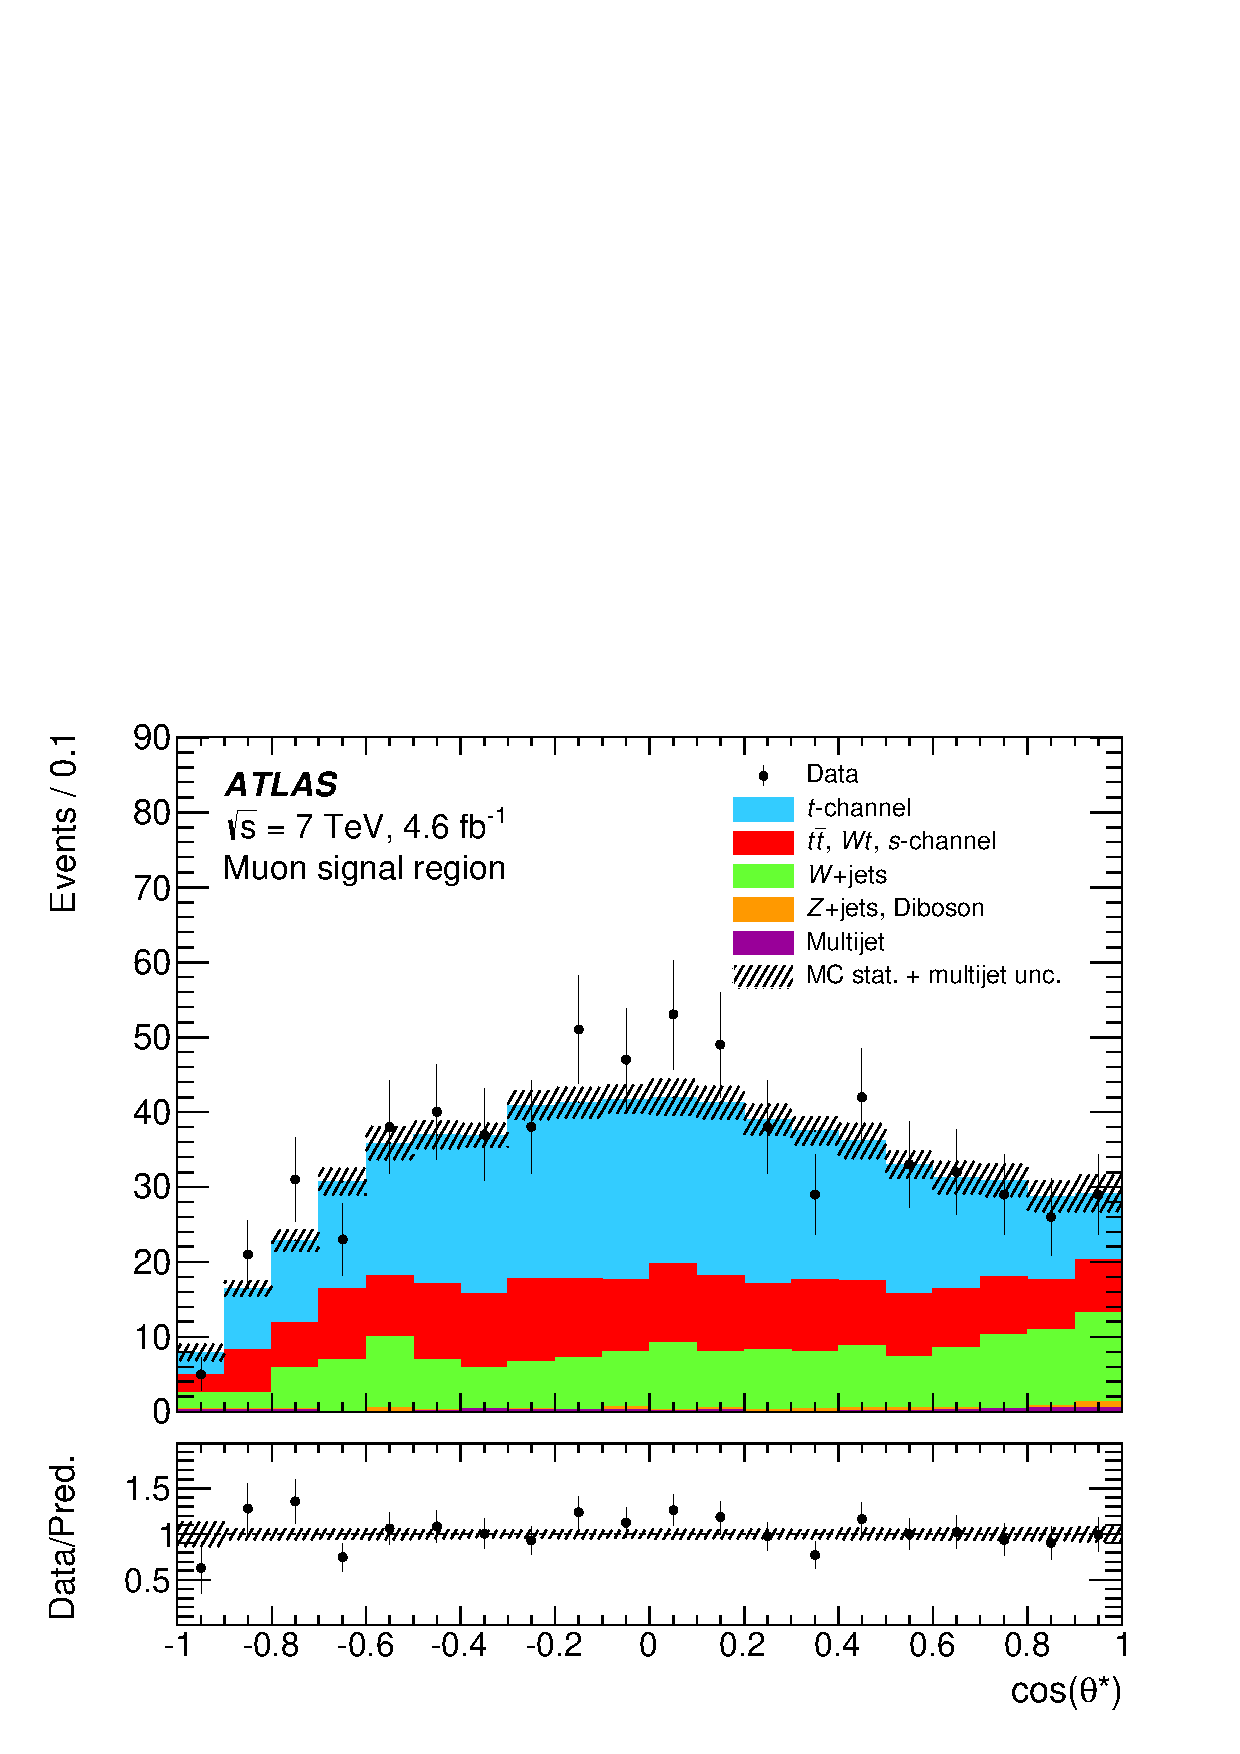
\includegraphics[width=0.29\textwidth]{atlas_anomcoupl/theta.pdf}\\(a)}\parbox[t]{0.3\textwidth}{\centering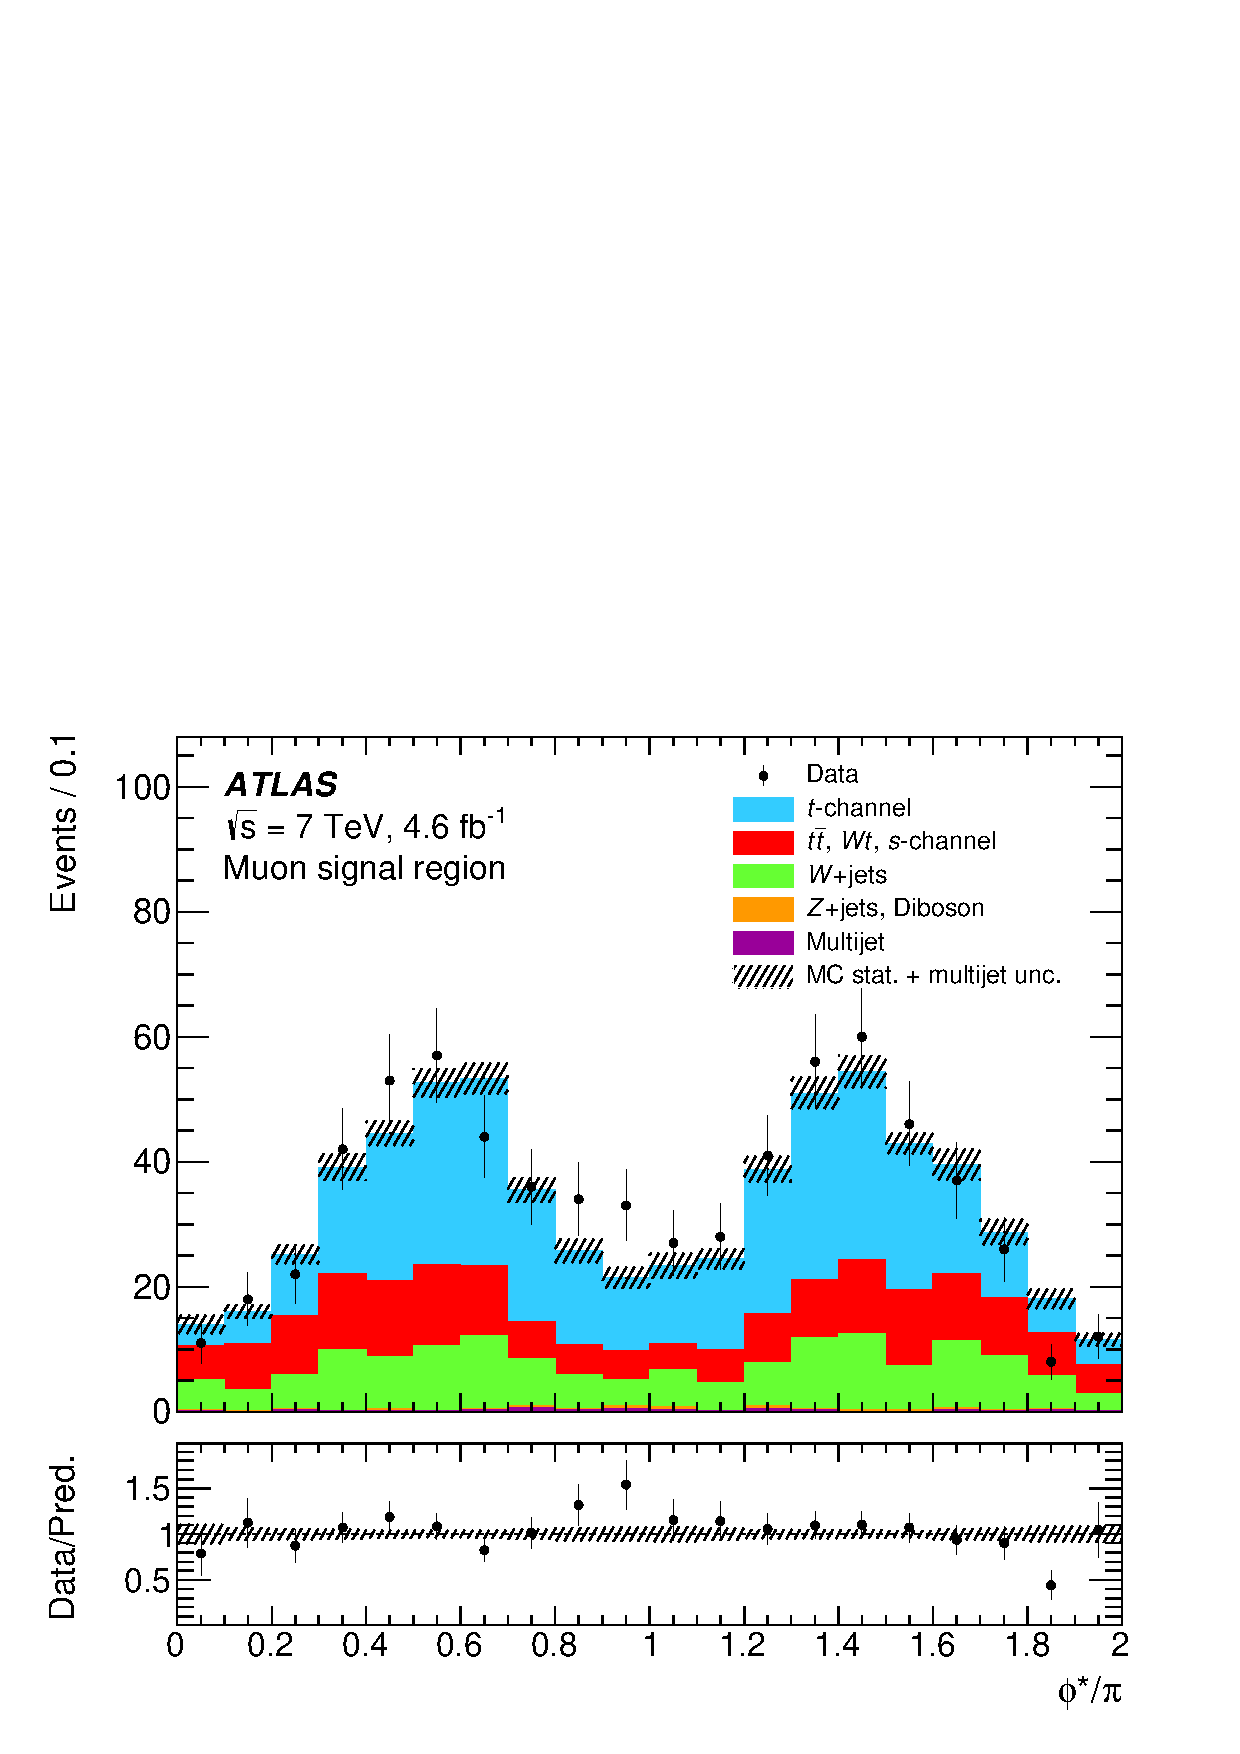
\includegraphics[width=0.29\textwidth]{atlas_anomcoupl/phi.pdf}\\(b)}\parbox[t]{0.38\textwidth}{\centering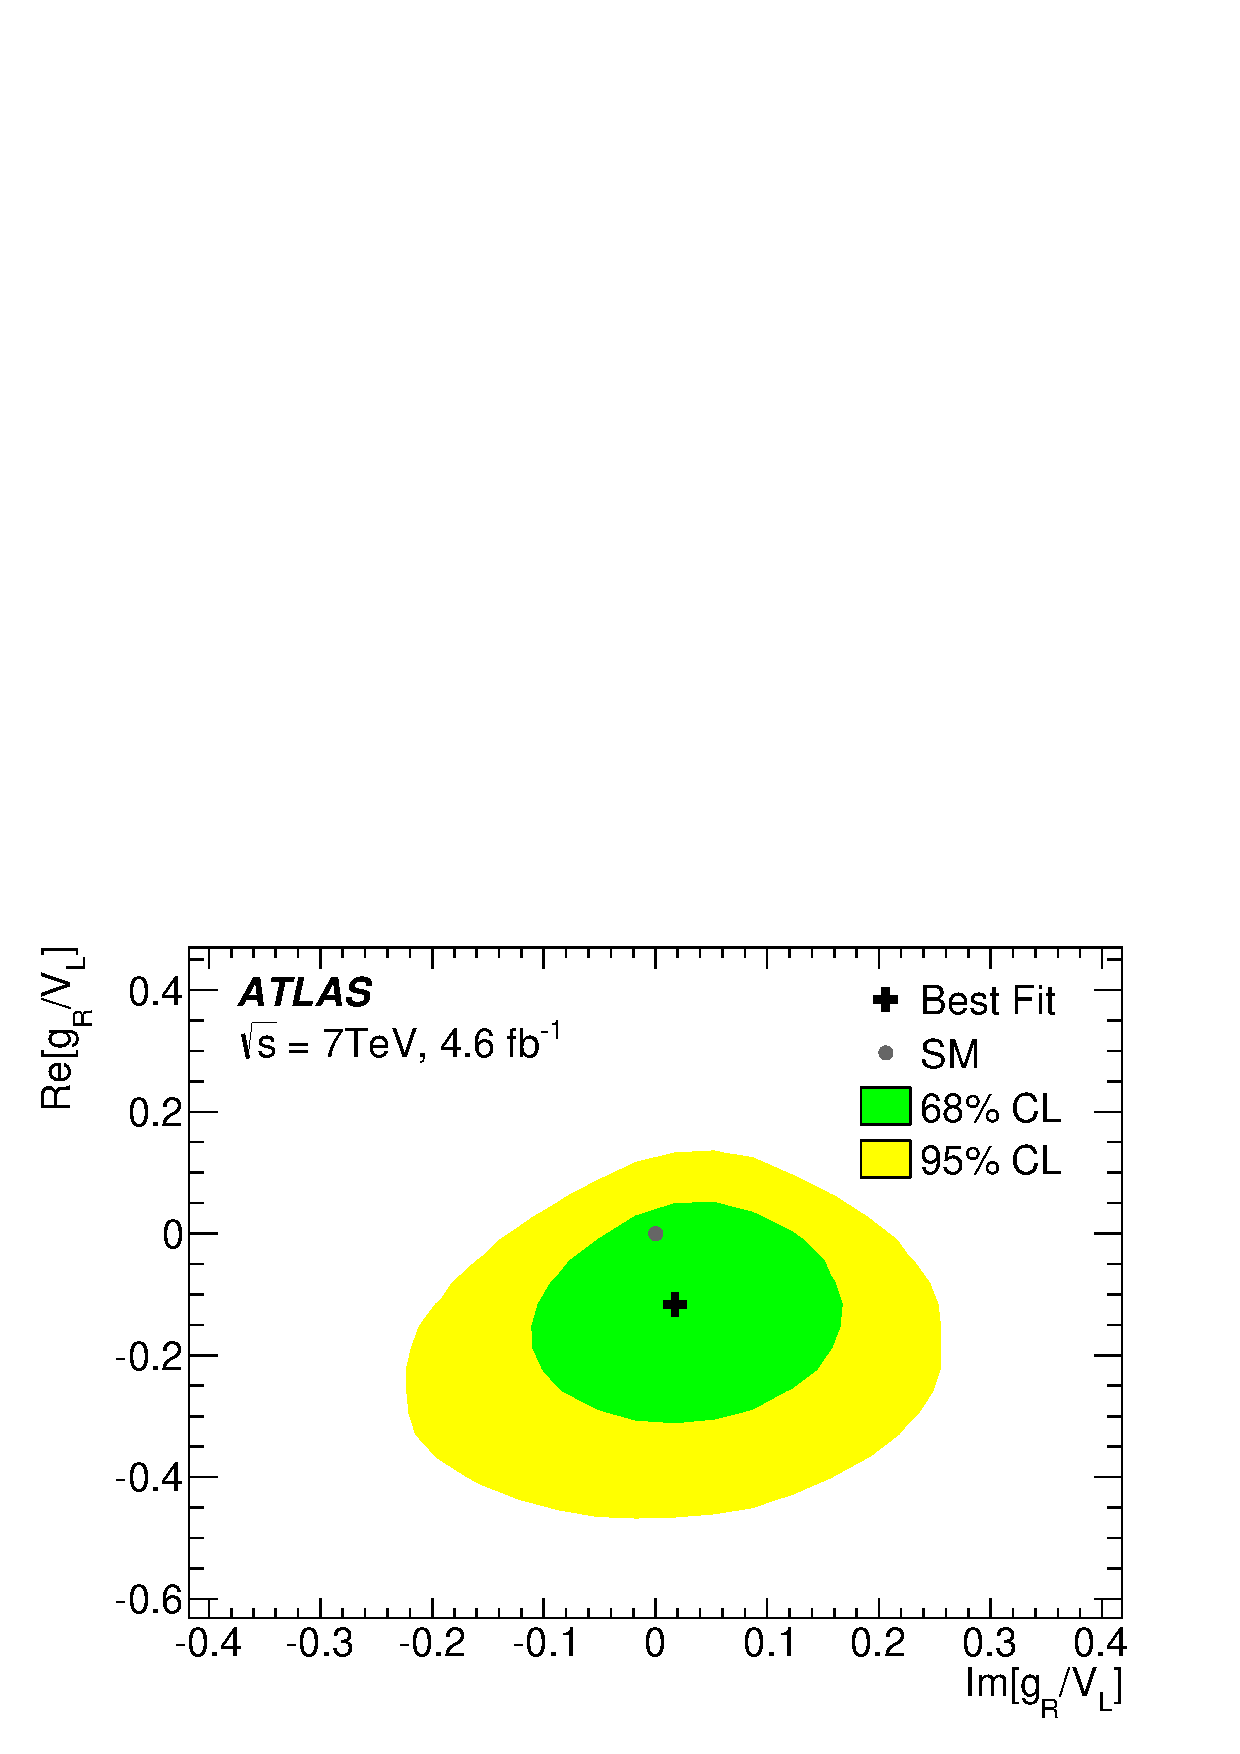
\includegraphics[width=0.36\textwidth]{atlas_anomcoupl/limits.pdf}\\(c)}
\end{center}
\caption{Limits on anomalous couplings~\cite{atlas-anomcoupl}.}
\end{figure}

\section{...}
\begin{figure}[htbp]
\begin{center}
\parbox[t]{0.40\textwidth}{\centering\includegraphics[width=0.35\textwidth]{cms_xsec13/mu2j1t.pdf}\\(a)}\parbox[t]{0.55\textwidth}{\centering\includegraphics[width=0.48\textwidth]{cms_xsec13/xsec.pdf}\\(b)}
\end{center}
\caption{Measurement of single top cross section at 13~TeV~\cite{CMS-PAS-TOP-15-004}.}
\end{figure}

\begin{thebibliography}{99}

\bibitem{atlas-anomcoupl}{Aad, Georges et. al., \emph{Search for anomalous couplings in the $Wtb$ vertex from the measurement of double differential angular decay rates of single top quarks produced in the $t$-channel with the ATLAS detector}, 
\texttt{arXiv:1510.03764[hep-ex]}, 2015.}

\bibitem{CMS-PAS-TOP-15-007}{CMS Collaboration, \emph{Fiducial t-channel single top-quark cross section at 8 TeV}, Tech. Rep. CMS-PAS-TOP-15-007, 2015.}

\bibitem{CMS-PAS-TOP-15-004}{CMS Collaboration, \emph{Measurement of the t-channel single top-quark cross section at 13 TeV}, Tech. Rep. CMS-PAS-TOP-15-004, 2015.}

\end{thebibliography}

\end{document}
